\documentclass[english]{scrartcl}

\title{Interim Report: Riyadh Metro}
\subtitle{v0.0}
\author{Phil Chodrow, Zeyad Al-awwad, and Shan Jiang}
\date{November 21, 2015}

\usepackage[T1]{fontenc}
\usepackage[utf8]{inputenc}
\usepackage{babel}
\usepackage{blindtext}
\usepackage{amsmath}
\usepackage{amsthm}
\usepackage{amsfonts}
\usepackage{amssymb}
\usepackage{graphicx}
\usepackage{booktabs}

\setkomafont{disposition}{\normalfont\bfseries}

\newtheorem{thm}{Theorem}
\newtheorem{lm}{Lemma}
\newtheorem{cor}{Corrolary}
\newtheorem{clm}{Claim}
\newtheorem*{thm*}{Theorem}
\newtheorem*{lm*}{Lemma}
\newtheorem*{cor*}{Corrolary}
\newtheorem*{clm*}{Claim}

\newcommand\abs[1]{\left|#1\right|}
\newcommand\E[0]{\mathbb{E}}
\newcommand\R[0]{\mathbb{R}}


\begin{document}

\maketitle

\section{Introduction}
	The purpose of this document is to outline progress to date on a multiplex approach to the Riyadh Metro project. \textbf{We hypothesize} that the availability of detailed network data and travel demand will lead to qualitatively different multiplex effects when compared to the mean-field, uniform demand model discussed by Strano et al.   
\section{Single-layer effects}
	Before analyzing multiplex effects, we begin with an analysis of the role of detailed traffic information on the street network alone. We will see that detailed traffic information has the following effects:
	\begin{enumerate}
		\item Nonuniform edgeweights -- speed limits and congestion estimates--lead to qualitatively similar shortest path distributions.
		\item Weighting by travel demand again leads to qualitatively different shortest path distributions and distributions of betweenness centrality. 
	\end{enumerate}
	\subsection{Impact of edge weights}
		\subsubsection{Shortest path distributions}

			Strano et al. used uniform edgeweights, with the weight of an edge proportional to its geographical length. PC had hypothesized that using nonuniform edgeweights -- reflecting either free flow or congested traffic conditions -- would significantly change the distributions of shortest path lengths and betweenness centrality. This appears to not be the case.   
			\begin{figure}
				\begin{minipage}{0.65\textwidth}
				% \centering
					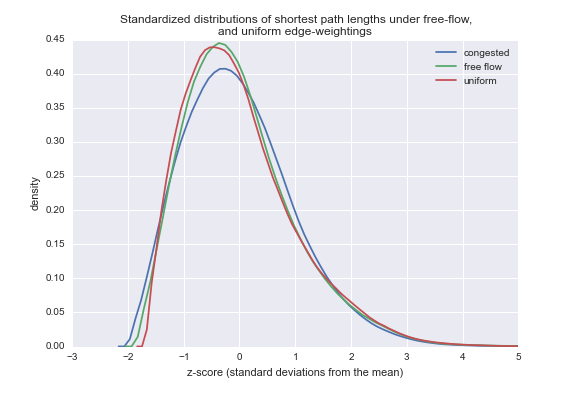
\includegraphics[width = 1\textwidth]{shortest_path_distributions_normed.png}
				\end{minipage}
				\begin{minipage}{0.25\textwidth}
					% \centering
						\begin{tabular}{llr}  
							\toprule
							Weighting    & $\mu$ (m) & $\sigma$ (m) \\
							\midrule
							Uniform     &  28.0   &  15.9 \\
							Free flow   &  16.7   &  8.5  \\
							Congested   &  19.8   &  9.5  \\
							\bottomrule
						\end{tabular}		
				\end{minipage}
				\caption{Normalized distributions of shortest paths under uniform, free flow, and congested edge weighting. The normalized distributions of shortest path lengths are almost identical under uniform and free flow edge-weighting, while the introduction of congestion leads to a slightly different shape.}
				\label{fig:1}
			\end{figure}
			

			This appears not to be the case. The normalized distribution of shortest path lengths and in the street network under uniform demand is shown in Figure \ref{fig:1} (left). Location and scale parameters are on the right. Contrary to PC's expectations, the distributions appear to share an underlying shape, with uniform and free flow distributions being especially close. The congested distribution appears to be slightly shifted. The parameters for the three cases deserve comments. Notably, the distributions all appear to be similar to those discovered in Strano et al, Fig. 1(c). 
			\begin{enumerate}
			 	\item Uniform edge weights lead to the slowest paths, since agents cannot optimize their trip by traveling on high-speed edges. 
			 	\item Free flow edge weights lead to the fastest paths, since agents can make unfettered use of high-speed edges such as highways. 
			 	\item Congested edge weights still allow agents to use high-speed edges; however, particularly desirable edges will have higher weights than in the free-flow case since other agents also wish to use them. 
			\end{enumerate} 
		\subsubsection{Betweenness centrality}
			Betweenness centrality is an estimate of the congestion at a node under uniform demand, under the assumption that agents traverse the shortest path from origin to destination. As before, we will see that different edge-weightings lead to different distributions, but the effects are not strongly pronounced. 
			\begin{figure}
				\centering
					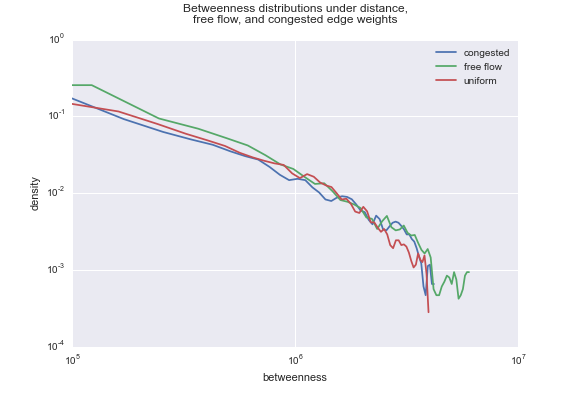
\includegraphics[width = 0.8\textwidth]{betweenness_distributions.png}
				\caption{Log-log plot of the distribution of betweenness centrality under congested, free flow, and uniform edge weightings}
				\label{fig:2}
			\end{figure}
			Figure \ref{fig:2} shows the distribution of betweenness centrality under each edge-weighting, plotted on log-log axes. The distribution in the uniform case falls off the fastest. Intuitively, this reflects the fact that, since all edges have the same speed, agents prefer those which are geographically closest. The result is that high centrality clusters in the approximate topological center of the network (cf Figure \ref{fig:3}, left).
			\begin{figure}
				\begin{center}
					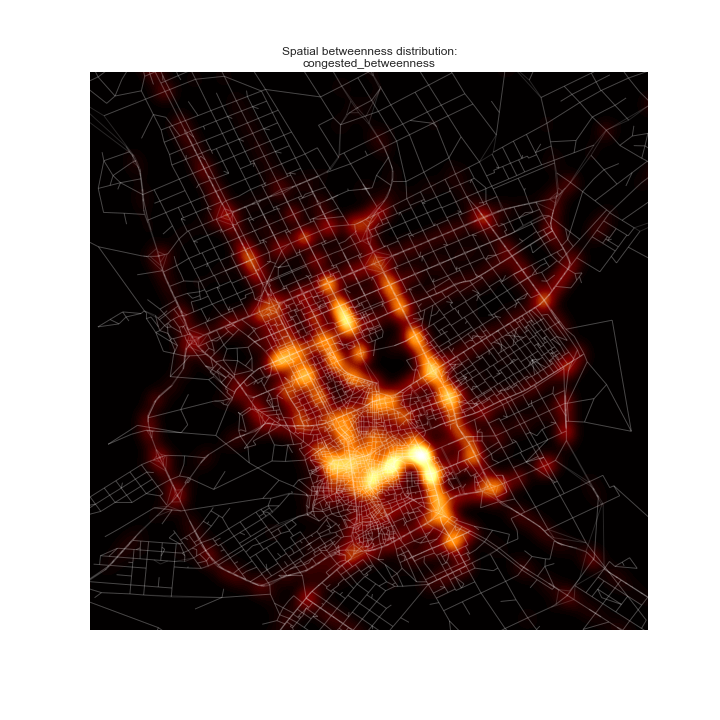
\includegraphics[scale = 0.2]{betweenness_spatial.png}
				\end{center}
				\caption{Spatial distribution of betweenness centrality under uniform edge weights (left), free-flow edge weights (center), and congested edge weights (right).}
				\label{fig:3}
			\end{figure}
			 In contrast, the free-flow case presents the opposite phenomenon, with a a small number of nodes having very high centrality. These nodes are those at the intersections of major thoroughfares (cf Figure \ref{fig:3}, center), though still clustering in the geographic center. Finally, betweenness under congested edge weights falls off less quickly than the uniform case, but does not have the extremely high concentration of the free-flow case. This reflects the impact of congestion effectively lowering the speed limits at high-demand nodes, rendering them less attractive for routing decisions. This effect is visible in Figure \ref{fig:3} on the right, in which betweenness centrality again concentrates at major thoroughfares, but is more dispersed as agents seek alternative routes. 
			
			Another way to measure the dispersion of betweenness centrality is by distance from the network centroid (weighted by betweenness under uniform weighting). Figure \ref{fig:4} shows how the average betweenness falls off as a function of distance from the centroid. As expected, the uniform case has the highest concentration near to the city center, with a rapid drop-off up to a roughly 15km radius. On the other hand, the free flow and congested cases are comparably dispersed geographically and fall off approximately linearly with distance. 
			\begin{figure}
				\centering
					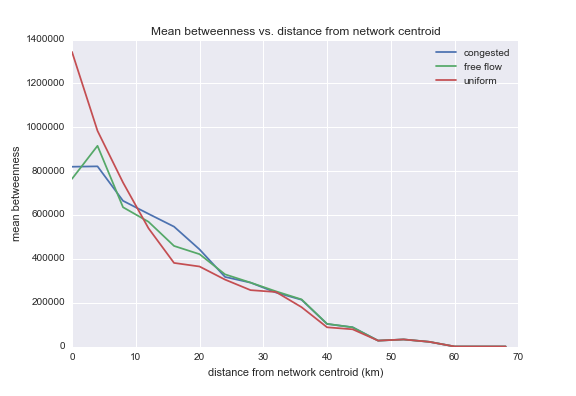
\includegraphics[width = \textwidth]{betweenness_dist.png}
				\caption{Average betweenness of nodes as a function of distance from the network centroid, under congested, free flow, and uniform edge weights}
				\label{fig:4}
			\end{figure}
			In summary: differential edge-weights alter the scale and location of shortest path distributions, and the geographical dispersion of betweenness centrality, but do not qualitatively change the behavior of the system. 

	\subsection{Impact of travel demand}

\section{Multiplex Effects}


\end{document} 

 